\section{Magic VLSI}

Jednym z bardziej popularnych oraz najbardziej dostępnych programów do projektowania układów scalonych
jest Magic VLSI\@.
Opracowany w 1983 roku przez Johna K. Ousterhouta i jego zespół na Uniwersytecie Kalifornijskim w Berkeley,
napisany w języku C, pierwotnie dla systemu Berkeley 4.2 będącego wariacją platformy Unix~\cite{MAGIC_article}.
Program ten posiada własną stronę internetową, na której można znaleźć dokumentację, kod źródłowy,
wskazówki dotyczące projektowania schematów, jak również pobrać program~\cite{MAGIC_site}.
Dzięki otwartemu kodowi źródłowemu, z czym wiąże się brak konieczności posiadania płatnej licencji,
oraz wysokiej funkcjonalności pozwalającej na pełne zaprojektowanie schematu układu scalonego,
Magic zyskał dużą popularność
w środowiskach akademickich i naukowych, a także wśród hobbystów.
Należy jednak zaznaczyć, że szeroka funkcjonalność programu
niekoniecznie sprzyja pozytywnym wrażeniom pierwszego użytkowania \textit{FTUE}
(ang. \textit{First Time User Experience}).
\newpage
\indent Unikalną cechą programu Magic jest wprowadzenie techniki strukturyzacji danych
zszytych narożników \textit{corner-stitched},
która znacząco poprawia jego wydajność.
Mechanizm ten opiera się na reprezentacji układu scalonego jako zestaw warstw,
na które składa się zestaw prostokątnych komórek.
%(ang. \textit{cells}).
Każda komórka zawiera zszyte narożnikami powierzchnie (ang. \textit{corner-stitched planes}),
opisujące jej geometrię oraz podkomórki, a każda z nich składa się z wielu prostokątnych kafelków.
Taka struktura pozwala na szybkie i efektywne operacje na schemacie,
takie jak znajdywanie wszystkich kafelek w danym obszarze lub sąsiadów danej komórki.
Dzięki zastosowanym mechanizmom możliwe jest także wykonywanie operacji na dużych obszarach
i szybką aktualizację danych.\\
\indent Magic posiada prosty interfejs graficzny,
który składa się z obszaru roboczego, paska menu oraz paska wyboru materiałów,
przedstawione na rys.~\ref{fig:magic_okno}.

\begin{figure}[h]
    \centering
    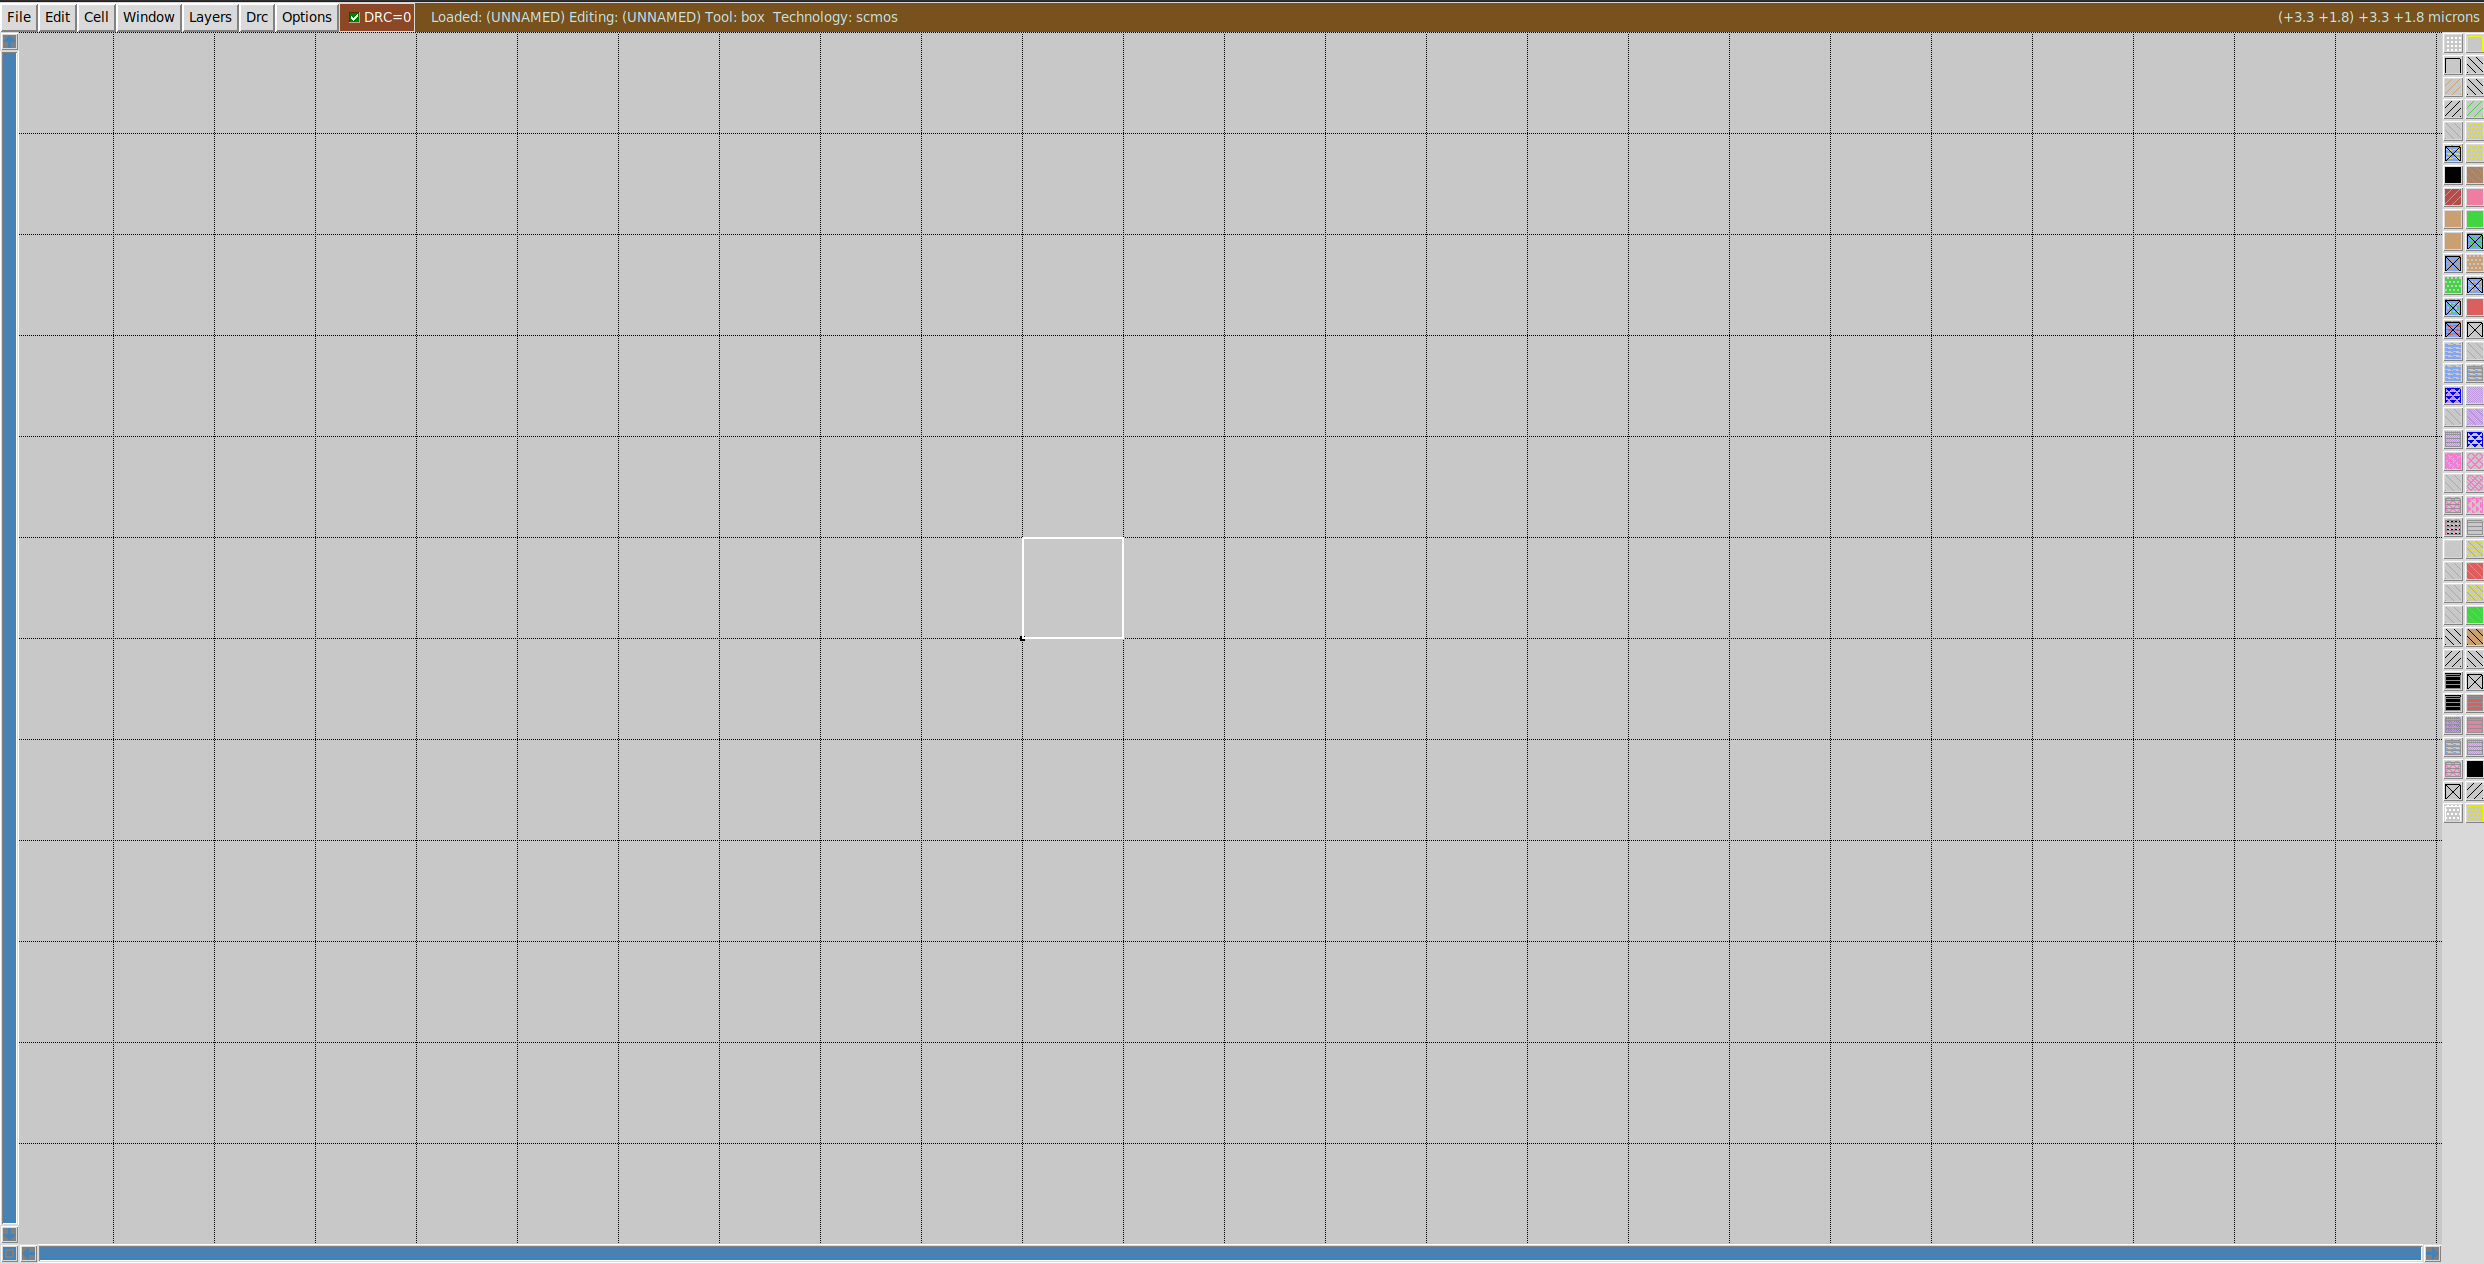
\includegraphics[width=.9\textwidth]{chapters/chapter2/img/magic_okno}
    \caption[Widok głównego okna programu Magic VLSI.]{Widok głównego okna programu Magic VLSI, źródło:~\cite{MAGIC_site}.}
    \label{fig:magic_okno}
\end{figure}

\indent Dodatkowo wraz z głównym oknem programu otwiera się okno konsoli pozwalające na wprowadzanie dodatkowych komend,
przedstawione na rys.~\ref{fig:magic_konsola}.

\begin{figure}[h]
    \centering
    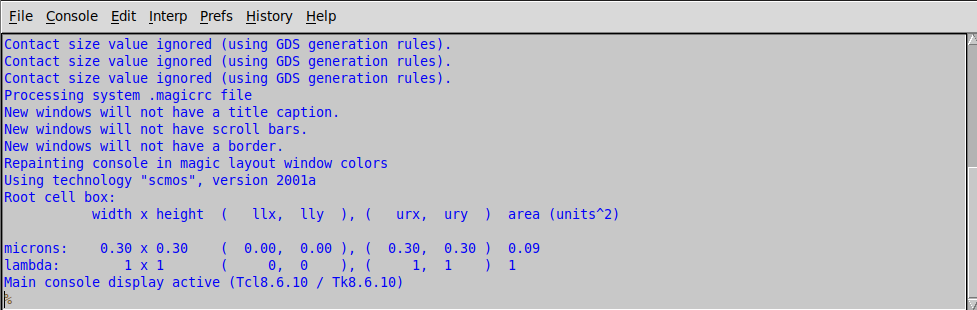
\includegraphics[width=.9\textwidth]{chapters/chapter2/img/magic_okno_konsola}
    \caption[Widok okna konsoli programu Magic VLSI.]{Widok okna konsoli programu Magic VLSI, źródło:~\cite{MAGIC_site}.}
    \label{fig:magic_konsola}
\end{figure}

\indent Rysowanie zaczyna się od zaznaczenia obszaru, lewy przycisk myszy służy do wyboru pozycji obszaru,
a prawy do jego rozszerzania.
Aby wypełnić obszar, należy wybrać odpowiedni materiał z paska wyboru
lub z już narysowanych komórek,
poprzez kliknięcie środkowym przyciskiem myszy.
Jest to początkowo nieintuicyjne dla użytkownika,
natomiast charakteryzuje się precyzją, stąd podobna funkcjonalność została zaimplementowana w projekcie.
W przypadku reszty funkcji takich jak przesuwanie, kopiowanie i skalowanie komórek,
jak również sama nawigacja po obszarze roboczym odbiega od obecnego standardu różnego rodzaju edytorów
i nierzadko wymaga wpisywania komend w konsoli.
Jest to obecnie rozwiązanie nieergonomiczne, gdyż obecnie większość podstawowych operacji wykonywanych jest
jedynie przy użyciu skrótów klawiszowych oraz myszy.\\
\indent Kolejnym istotnym aspektem jest także sama instalacja programu Magic VLSI\@.
Ze względu na pierwotne przeznaczenie programu dla systemu Unix,
jego instalacja na systemach Windows wymaga albo zainstalowania maszyny wirtualnej z systemem Linux,
albo skorzystania z dodatkowego narzędzia \textit{Cygwin}~\cite{MAGIC_site,cygwin}.
Zważając na dużo większą popularność systemów operacyjnych Windows~\cite{os_stats},
może być to niepotrzebną komplikacją dla użytkowników dopiero uczących się projektowania układów scalonych.\\
\indent Nadmienić jednak trzeb, że istotną zaletą programu Magic jest prosta szata graficzna,
a w szczególności tekstury materiałów, które są czytelne, pozwalają na łatwe rozróżnienie warstw,
nawet gdy się na siebie nakładają, dzięki dobrze dobranym wzorom i kolorom, przykład przedstawiono na rys. \ref{fig:magic_tran}.
Implementacja podobnego rozwiązania w projekcie poprawi czytelność schematów.

\begin{figure}[h]
    \centering
    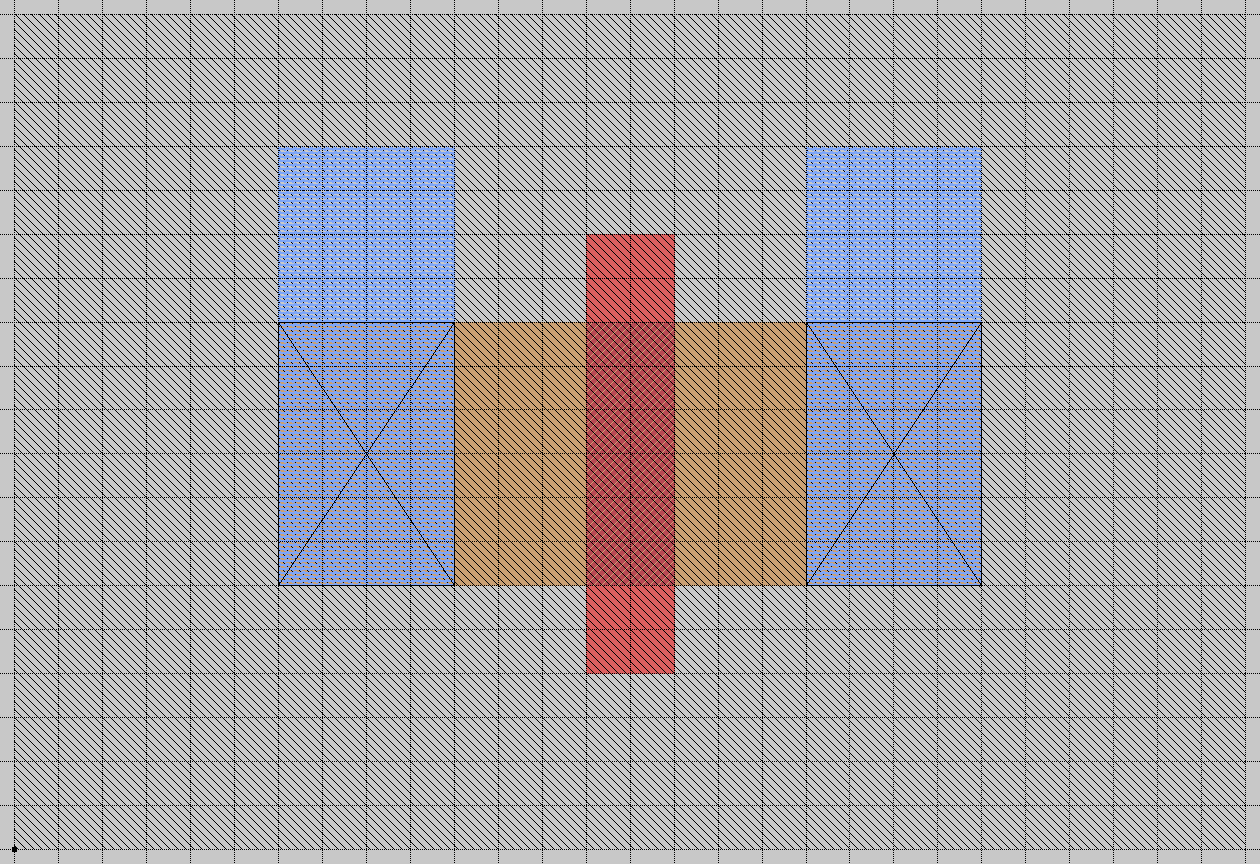
\includegraphics[width=.9\textwidth]{chapters/chapter2/img/magic_tran}
    \caption[Przykład tranzystora pMOS narysowanego w programie Magic VLSI\@.]
    {
        Przykład tranzystora pMOS narysowanego w programie Magic VLSI\@.
        Mimo nakładania się wielu warstw schemat jest dalej czytelny,
        nawet w miejscu połączenia warstw~\textit{metal1} i~\textit{pdiffusion} oraz warstwy~\textit{nwell},
        żródło: opracowanie własne.
    }
    \label{fig:magic_tran}
\end{figure}
